\paragraph{Мейн информация}
Файл представляет собой ELF-бинарник под x86\_64 Linux.
При запуске программа предлагает пользователю выбрать один из двух режимов:
\begin{itemize}
    \item \textbf{1. Encrypton} --- зашифровать флаг из файла \texttt{flag.txt} и сохранить в \texttt{encrypted\_flag.txt}
    \item \textbf{2. Decryption} --- расшифровать содержимое \texttt{encrypted\_flag.txt} и сохранить в \texttt{flag.txt}
\end{itemize}

Вход обрабатывается функцией \texttt{FUN\_001011a0}, основной управляющей логикой занимается \texttt{FUN\_00101460}.

\paragraph{Анализ шифрования}

Функция шифрования представлена в дизассемблированном виде в \texttt{FUN\_00101280}.
Она применяет к каждому байту входной строки позиционно-зависимое преобразование.
Ниже приведена соответствующая формула:

\[
    \text{encrypted} = (i \oplus ((c - 0x19) \oplus \sim 0x28)) + 0x48
\]

где:
\begin{itemize}
    \item $c$ — ASCII-код исходного символа
    \item $i$ — индекс символа в строке
\end{itemize}

Пример кода на C (упрощённо):
\begin{verbatim}
        char c = input[i];
        char encrypted = (i ^ ((c - 0x19) ^ ~0x28)) + 0x48;
\end{verbatim}

Элементы шифра:
\begin{itemize}
    \item используется XOR с битовой маской
    \item учитывается позиция символа
    \item добавлены константные смещения (+0x19, +0x48 и др.)
\end{itemize}

\paragraph{Анализ дешифрования}

Дешифрование реализовано симметрично в \texttt{FUN\_00101380}.
Формула обратного преобразования выглядит так:

\[
    \text{original} = (((c - 0x29 - 0x1F) \oplus \sim 0x28) + 0x19) \oplus i
\]

Эквивалентный код на C:

\begin{verbatim}
        char c = input[i];
        char decrypted = (((c - 0x48) ^ ~0x28) + 0x19) ^ i;
\end{verbatim}

Зашифрованный флаг, прочитанный из файла, преобразуется обратно в оригинальную строку и сохраняется в \texttt{flag.txt}.

\paragraph{Особенности}

\begin{itemize}
    \item Используется самодельный криптоалгоритм с симметричным ключом.
    \item Преобразование для меня очень запутано, но линейно и обратимо.
    \item Для использования этого алгоритма обязательно использовать txt файлы для инпута и аутпута.
\end{itemize}

\paragraph{Тестовый запуск}

\paragraph{}
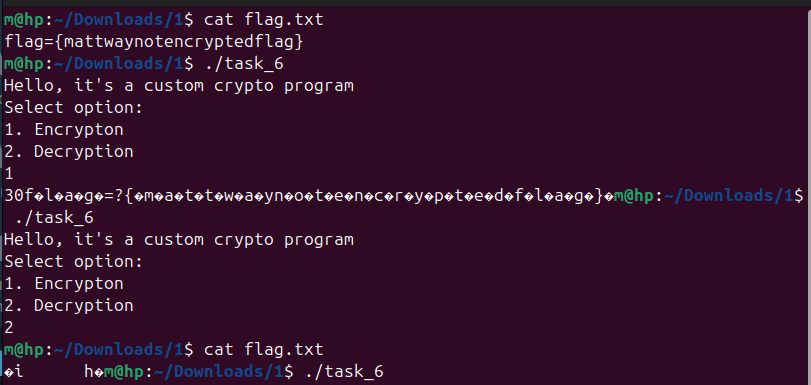
\includegraphics[width=1\linewidth]{static/_task_6}

Предполагаю, что я что-то сделал не так, поскольку формулы шифрации и дешифрации противопоставляют друг другу
